\chapter{Diagnostic tools using Machine Learning} \label{chap:sota}
\label{chap:chap2}
\section*{}

\section{Diagnostic tools} \label{Diagnostic}

\paragraph{}Neuroscientific technologies use experimental methods to study the patients' brain processes. Those methods include neuroimaging, psychophysical techniques or psychological tests which are used to study processes such as learning, attention, memory, or emotion \cite{Corchs2019}.
\espaco

The following methods stand out:

 
\begin{itemize}


\item Electroencephalogram (EEG)

Electroencephalography is a simple, non-invasive technique based on recording and evaluating brain activity using electrodes placed on the skull surface \citep{Avilov2020} \citep{Da2019}.The (EEG) is the record that results from the measurement of the electrical potentials of the brain \cite{Bender2015} \citep{Xu2020}. EEG shows the electrical fluctuation in the different locations of the cortex  \citep{Zheng2016}. However, it has the disadvantage of having an insufficient resolution to register the neuronal activity in deeper brain structures, such as the \textit{nucleus accumbens} related to the processing of emotions\cite{Lang2010}. %\citep{8701676}. 

Study using Mismatch Negativity (MMN) tomography technique resulting in classification of patients with DOC in figure \ref{ferramentaMMN}
\begin{figure}[ht!]
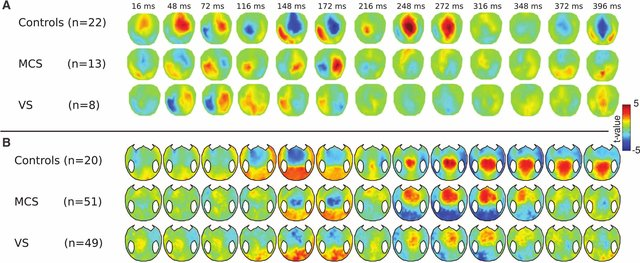
\includegraphics[scale=0.7]{figures/MMN-topography-in-patients-with-disorders-of-consciousness-and-in-healthy-controls-The_W640.jpg}
\caption[DOC patient's MNN topography versus healthy control patients]{ MMN topography in healthy controls patients versus DOC’s patients. Observation of t test maps (deviation and standard trials) in A  comparing with  similar maps obtained in France between 2008 and 2011\cite{King2011}
\cite{Boly2011}} %legenda imagem no indice e no texto
\label{ferramentaMMN}
\end{figure}

\item  (Functional) Magnetic Resonance

 It is a method of diagnosis and fundamental research in market research analysing emotions planning surgery brain mapping neurosciences \citep{fmri}. It allows the analysis of the subjects' response to different activities or stimuli. Magnetic resonance imaging is a non-invasive technique used to obtain information about the subjects' response to different stimuli (very common in research and analysis of neurological diseases such as Alzheimer's Disease and also for soft tissue injuries and inflammation). This technique evaluates the activation and the emotional state of the subject when exposed to certain stimuli \cite{noauthor_fmri_nodate}. 
 
 
\item  GSR (galvanic skin response)

Measurement of the galvanic response is done by placing
electrodes on the fingers. Studies measure resistance
skin and its conductance.

A GSR amplifier applies constant tension to the skin using low voltage that the individual cannot
perceive it through electrodes. The current generated in the
skin by tension can be detected and recorded. The output of the GSR amplifier determines the conductance.
The conductance of the skin gives feedback on the body's response to the stimulus; it is widely used in post-coma and coma phases
\cite{Altntop2021,Luaute2018}.



\item  Eye-tracking

 Eye-tracking refers to recording the movements of an individual's eye while examining a visual stimulus. In broad, it is responsible for measuring eye movements using a camera that quantifies them. Modern eye trackers record eye position and movement using contrast to locate the central point of the pupil and create a reflection of the cornea using infrared light. It is possible to analyse of the position of the gaze and the movement of the eyes in three-dimensional environments \citep{Taherkhani2012}.
Eye-tracking techniques apply to domains where interaction and interests matter,
looking to sell or immerse to improve the customer or user experience. In medicine, it is essential to recognize behaviours and patterns to investigate further and characterize\cite{Ting2014}.


\item  Face reading

 Facial expressions are one of the most robust  visual methods for conveying emotions. The face plays a crucial role in the cognitive processes of individuals, since the signs that show facial expressions denote internal states or emotions. The analysis of facial expressions provides valuable information when combined with other tools that allow sensory information collection, such as eye-tracking or EEG.

\end{itemize}

\section{General idea of application}
It is common in health areas such as medicine and biomedical to have pre-determined datasets for training and a new dataset(s) for testing.
Typical general use case: Models based on the knowledge of n patients, trying to classify the status of other patients who will arrive \citep{MULLER2019145}.

It is common in medical science to have pre-determined datasets for training and a new dataset(s) for testing.		
A typical use case is, for instance, a model based on the knowledge of n patients, trying to classify the status of other patients who will arrive \citep{MULLER2019145}.		
The raise of high-performance computing (which includes GPU's, CPU's, high-speed interconnect, memory, libraries, storage, compilers, etc.) 	
increased the speed of algorithms that would generally take months to be completed, even at a distance, as in the case of cloud computing. \ref{Cc} \cite{ai}.
